\documentclass[tikz,border=3pt]{standalone}
\usepackage[utf8]{inputenc}
\usepackage[T1]{fontenc}
\usepackage{lmodern}
\renewcommand{\familydefault}{\sfdefault}
\usepackage{sansmath}\sansmath
\usepackage{chemfig}
\usepackage{pgfplots}\pgfplotsset{compat=1.18,/pgf/number format/use comma,/pgf/number format/1000 sep={.}}
\usetikzlibrary{arrows.meta,calc,positioning,decorations.pathmorphing,patterns}
% paleta del sitio
\definecolor{nar}{HTML}{E8680C}\definecolor{narc}{HTML}{FFB35C}\definecolor{hielo}{HTML}{FFF3E8}
\definecolor{tinta}{HTML}{1D1D1F}\definecolor{gris}{HTML}{6E6E73}\definecolor{lila}{HTML}{7C5CF0}
\definecolor{azul}{HTML}{2F6FD6}\definecolor{menta}{HTML}{17A673}\definecolor{coral}{HTML}{E8342A}
\begin{document}
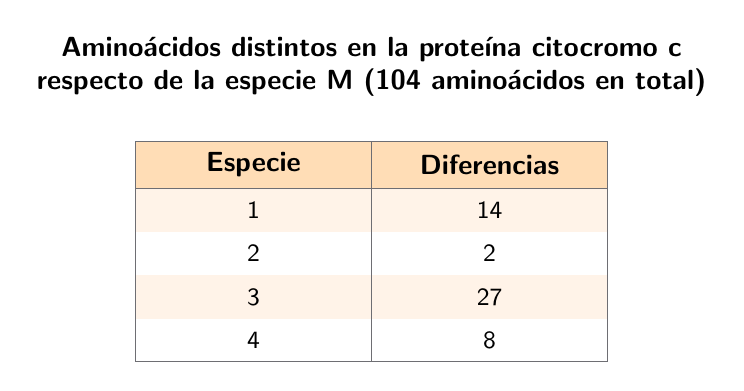
\begin{tikzpicture}[font=\small]
\node[font=\bfseries,align=center] at (3,0.95) {Aminoácidos distintos en la proteína citocromo c\\respecto de la especie M (104 aminoácidos en total)};
\fill[narc!45] (0,0) rectangle (6,-0.6);
\node[font=\bfseries] at (1.5,-0.3) {Especie};
\node[font=\bfseries] at (4.5,-0.3) {Diferencias};
\foreach \e/\d [count=\i] in {1/14,2/2,3/27,4/8}{
  \pgfmathsetmacro{\y}{-0.6-0.55*\i}
  \ifodd\i \fill[hielo] (0,\y) rectangle (6,\y+0.55); \fi
  \node at (1.5,\y+0.275) {\e};
  \node at (4.5,\y+0.275) {\d};}
\draw[gris] (0,0) rectangle (6,-2.8);
\draw[gris] (3,0) -- (3,-2.8);
\draw[gris] (0,-0.6) -- (6,-0.6);
\end{tikzpicture}
\end{document}
